\documentclass[11pt, a4paper]{article}
\usepackage[a4paper, total={6.5 in,9in}]{geometry}
\usepackage[slovene]{babel}
\usepackage[utf8]{inputenc}
\usepackage[T1]{fontenc}
\usepackage{lmodern}
\usepackage{amsmath}
\usepackage{ amssymb }
\usepackage{amsfonts}
\usepackage{amsthm}
\usepackage{comment}
\usepackage{url}
\usepackage{gensymb}
\usepackage{subcaption}
\usepackage[pdftex]{graphicx}
\usepackage[section]{placeins}
\usepackage{mathtools}
\usepackage{float}
\usepackage{epstopdf}
\renewcommand{\vec}[1]{\mathbf{#1}}
\usepackage{hyperref}
\usepackage{wrapfig}
\usepackage{mhchem}
\pagestyle{plain}

\begin{document}

    \begin{center}
    {\LARGE\bfseries 7. Nelinearni in razdelčni modeli\par}
    \vspace{1cm}
    
    {\Large Domača naloga pri predmetu Modelska analiza I\par}
    \vspace{0.2cm}
    {\normalsize Avtor: Matic Noč \par}
    \vspace{0.2cm}    
    {\normalsize 15.11.2017 \par}    

    
    \end{center}
\section{Uvod}
Obravnavali bomo problem nelinearnega luščenja parametrov. Enačb za minimum residualov v tem primeru ne moremo analitično rešiti, kot smo to lahko naredili v primeru linearnih modelov, temveč moramo uporabiti numerično minimizacijo, za katero lahko uporabimo gradientno ali Newtnovo metodo, ki nam poiščeta minimum $\chi^2$. Videli bomo, da je v določenih primerih uspešnost minimizacije zelo pogojena s začetnim približkom, še posebej, ko imajo funkcije velike gradiente (npr. eksponentna). Pogledali si bomo tudi razdelčne modele, ki se jih gradi v medicini, za opis transporta tekočine iz določenih organov in ga opišemo s sklopljenimi diferencialnimi enačbami, ki jih rešimo in nato iščemo parametre modela za kasnejše napovedovanje.
\section{Nelinearni odziv tkiva na reagente (naloga 6.)}
Tokrat zopet obravnavamo odziv tkiva na reagent, ki ga lahko zapišemo v obliki kemijske reakcije


\begin{equation}
\ce{Y + X <=>Y^*}.
\end{equation}
V stacionarnem stanju tako dobimo zvezo
\begin{equation}
y=\frac{y_0x}{x+a},
\end{equation}
kjer pomeni $y_0$ nasičeni odziv tkiva in $a$ koncentracijo, potrebno za odziv, ki je enak polovici nasičenega. V enačbi dodamo še en člen $p$, ki nam doda novo prostostno stopnjo in opisuje neposredno moč vpliva reagenta na odziv tkiva, za razliko od prejšne, ko je bil vpliv posreden, preko konstant in razmerij.
\begin{equation}
y=\frac{y_0x^p}{x^p+a^p},
\end{equation}
Dobili smo nelinearni model, ki ga ne moremo linearizirati. Zapišimo cenovno funckijo $\chi^2$
\begin{equation}
\chi^2 = \sum \frac{(y_i - f(x_i, y_0,a,p))^2}{\sigma^2}
\end{equation}
Iščemo minimum $\chi^2$, zato zapišemo enačbe
\[
\partial/\partial y_0 (\chi^2) = 0
\]
\[
\partial/\partial a (\chi^2) = 0
\]
\[
\partial/\partial p (\chi^2) = 0
\]
V splošnem bo to sklopljen nelinearni sistem enačb, ki ga ne moremo analitično rešiti, zato se bomo problema lotili s numeričnim iskanjem minimuma $\chi^2$.
\subsection{Numerično iskanje minimuma $\chi^2$}
Na voljo imamo vse optimizacijske metode, ki iščejo minimum funckije, vendar pa bomo izkoristili dejstvo, da je $\chi^2(x,\vec{a})$ v okolici minimuma parabola, torej jo lahko razvijemo do drugega reda in zapišemo pogoj za minimum v obliki gradienta. Seveda daleč stran od minimuma, ta približek ne bo dober in bo boljše uporabiti kar gradietno metodo približevanja v nasprotni smeri največjega narašačanja, da se bomo hitreje bližali minimumu. Metoda je precej občutljiva na začetni približek, saj se lahko hitro ujame v lokalne minimume in ne vsebuje nekih mutacij oziroma simuliranega ohlajanja, ki bi nas potegnili ven iz minima. Zapišimo torej gradientno metodo
\begin{equation}
 \mathbf {a} _{n+1}=\mathbf {a} _{n}-\gamma \nabla \chi^2(\mathbf {a} _{n}),
 \end{equation}
razumemo jo predvsem intuitivno. Ker je gradient smer največjega narašačanje funckije v dani točki, bo v nasprotni smeri zagotovo nek minimum (ki pa je lahko tudi lokalni). Gradient pomnožimo s konstantno $\gamma$, ki pomeni kako močno bomo segli v nasprotni smeri gradienta, in se skozi iteracije prilagaja, in se manjša, ko se manjšajo razlike med novim in starim približkom. Kot si predstavljamo bo v okolici minimuma metoda počasna, saj se gradieti ne razlikujejo kaj dosti, problematična pa je tudi izbira $\gamma$. \newline\newline
\subsection{Newtnova optimizacijska metoda}
Razvijmo našo funkcijo $\chi^2$ do drugega reda.
\begin{equation}
f(x_{n}+\Delta x)\approx f(x_{n})+f'(x_{n})\Delta x+{\frac {1}{2}}f''(x_{n})\Delta x^{2}
\end{equation}
Iščemo stacionarno točko, torej tam kjer bo $ f(x_{n}+\Delta x) = f(x_{n})$ oziroma bo odvod v smeri premika enak 0.
\begin{equation}
 0={\frac {\rm {d}}{\rm {d\Delta x}}}\left(f(x_{n})+f'(x_{n})\Delta x+{\frac {1}{2}}f''(x_{n})\Delta x^{2}\right)=f'(x_{n})+f''(x_{n})\Delta x.
\end{equation}
\begin{equation}
 x_{n+1} = x_n - \frac{f'(x_n)}{f^{''}(x_n)}
\end{equation}
v več dimenzijah je namesto odvodov potrebna jakobijeva matrika oziroma gradienti 
\begin{equation}
\mathbf {x} _{n+1}=\mathbf {x} _{n}-\gamma [\mathbf {H} f(\mathbf {x} _{n})]^{-1}\nabla f(\mathbf {x} _{n}).
\end{equation}
Algoritem, ki združuje obe metodi se imenuje $Levenberg-Marquardtov$ algoritem in preklaplja med gradientno in newtnovo metodo ter sproti prilagaja faktor $\gamma$ in se ustavi, ko doseže lokalni minimum oziroma se funkcija z iteracijami ne razlikuje več.
\subsection{Rešitev}
 \begin{figure}[H]
\hspace*{-2.5cm}  
  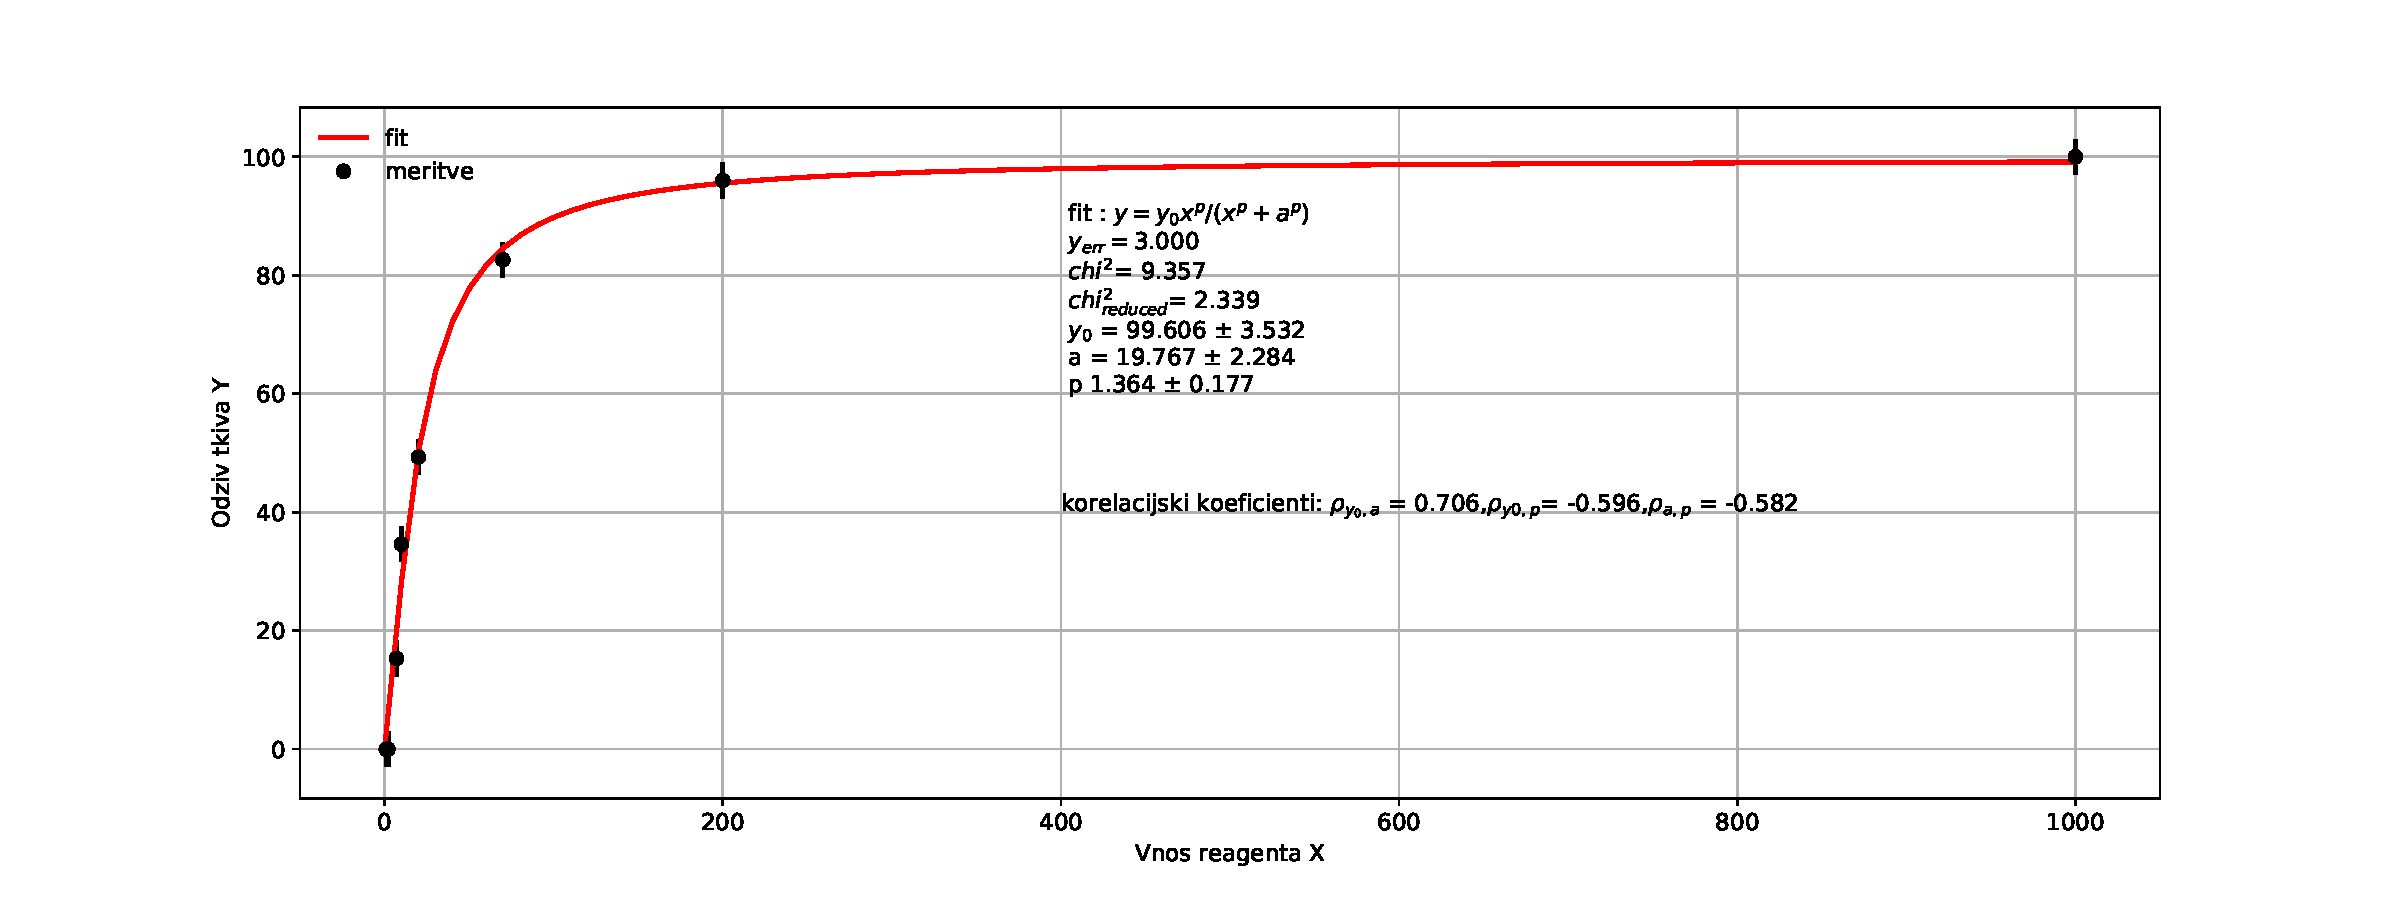
\includegraphics[width=20cm]{prva_fit.pdf}
 \caption{Razširjen model odziva tkiva na reagent. \textbf{Vidimo, da se je proti prejšnem modelu $\chi^2$ zmanjšal iz 13 na 9 in sedaj predstavlja glede na reduciran $\chi_{reduced}^2$ bolj optimalno vrednost, kot je brez parametra $p$, kar je smiselno in statistično upravičeno}. Izračunal sem tudi korelacijske koeficiente, in napake, parametrov iz korelacijske matrike, ki jo algoritem poda, kot $H^{-1}$, ki jo izračuna kot aproksimacijo iz $H = J^TJ$, pri čemer je $J$ jakobijeva matrika v zadnji iteraciji. Za konvergenco je optimziacija potrebovala le 25 iteracij. Podal sem tudi \textbf{korelacijske koeficiente}, ki nam povedo kako korelirani so naši parametri. Vidimo, da sta oba $y_0$ in $a$ antikorelirana s $p$, med tem ko sta $y_0,a$ korelirana.}
\end{figure}
\begin{figure}[H]
\hspace*{-2.5cm}  
  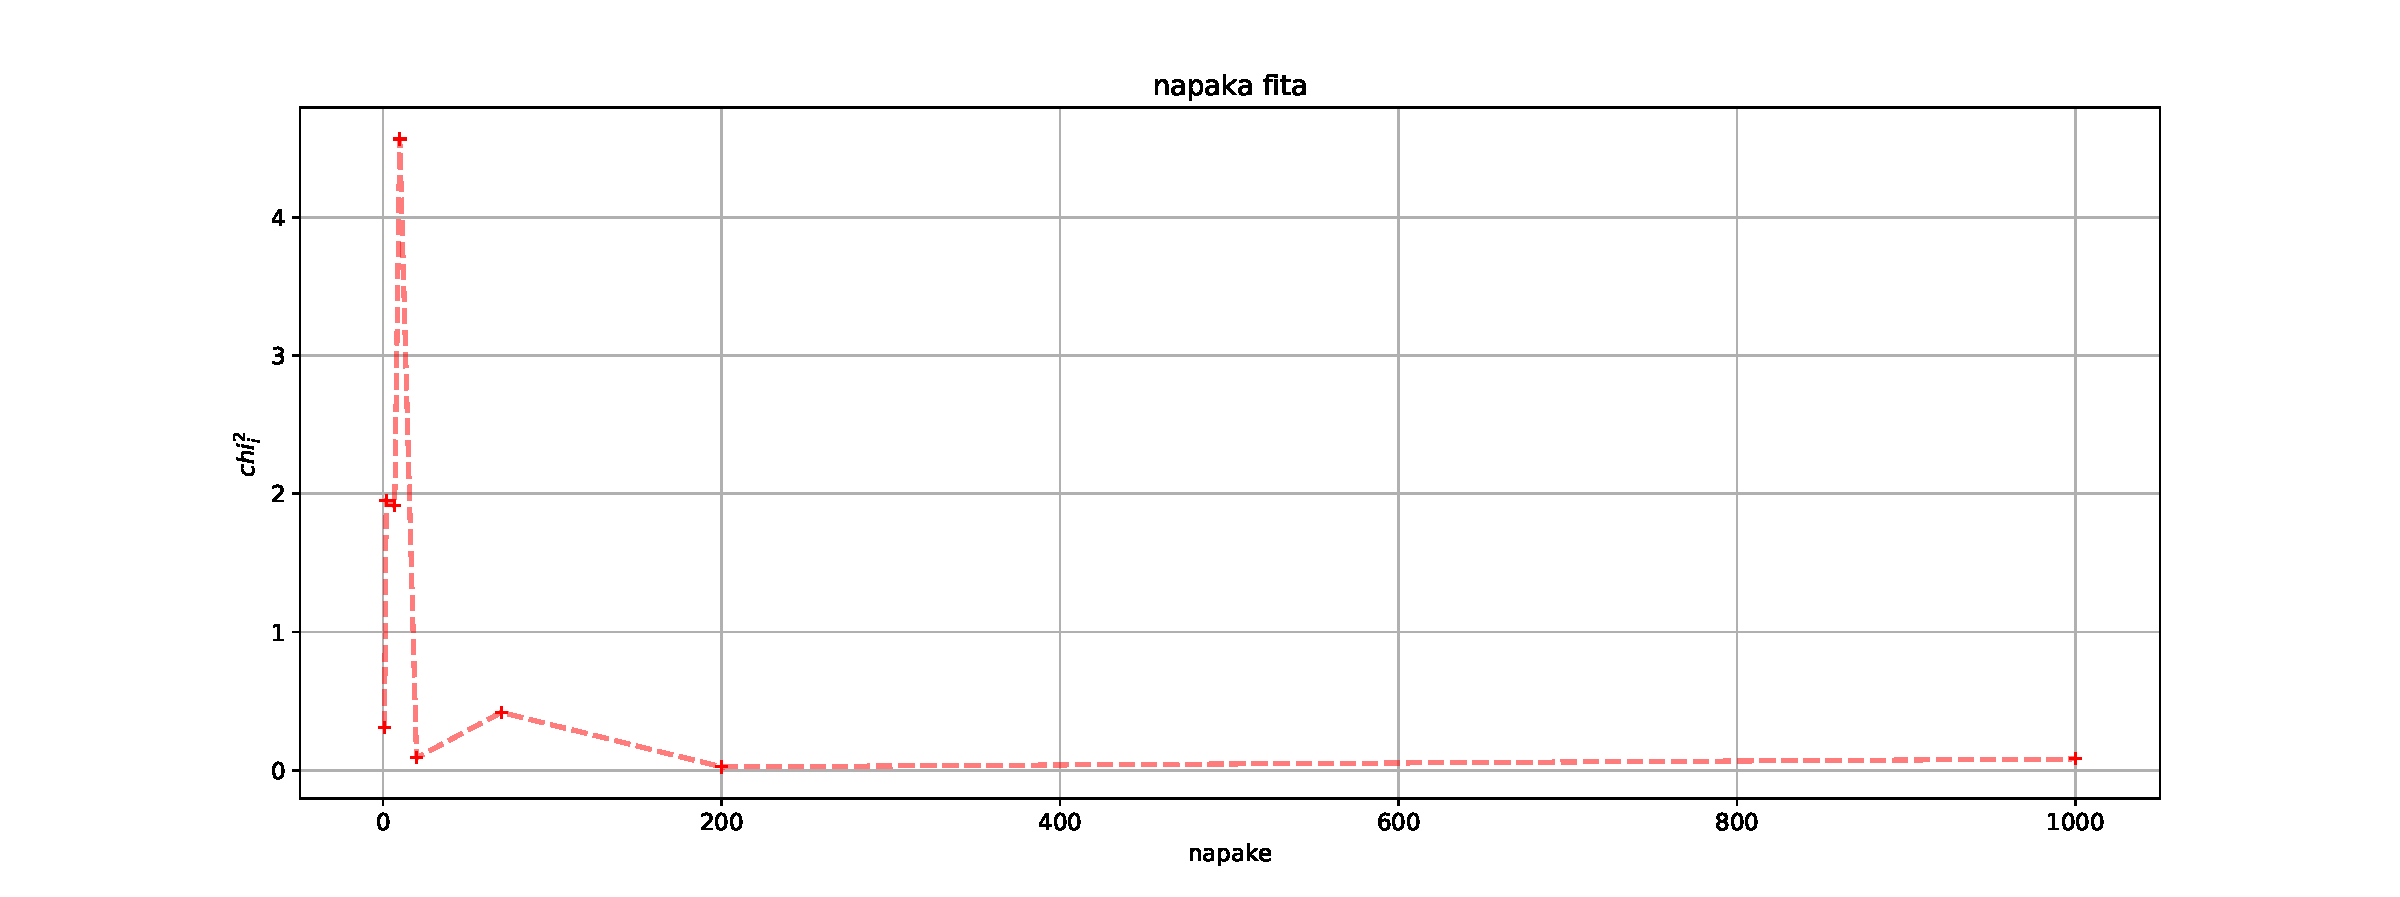
\includegraphics[width=20cm]{prva_napaka.pdf}
 \caption{Napake niso enakomerno razporejene, kar kaže na to da se da naš model še izboljšati.}
\end{figure}

\section{Razdelčni modeli}
\subsection{Kompartmenti}
Razdelki oziroma kompartmenti je fiziološki pogled na človeško telo, ki je pretežno sestavljeno iz tekočine in ga zato lahko namesto sklopov organskih sistemov opišemo s kompartmetni, med katerimi poteka pretok in difuzija. Tako se razdeli telo na tekočino znotraj celic, tekočino zunaj celic in medcelično tekočino, in se s pretoki s pomočjo različnih kanalov praktično razloži celotno človeško fiziologijo.\newline\newline

 \begin{figure}[H]
   
  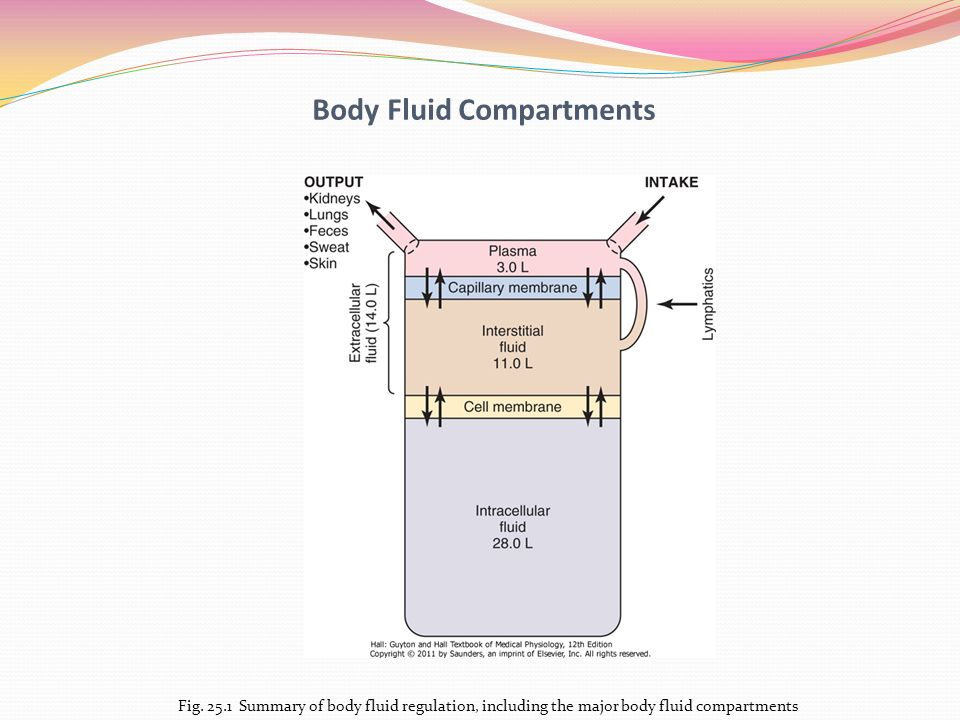
\includegraphics[width=16cm]{compartment.jpg}
 \caption{Kompartmenti v telesu. vir : http://slideplayer.com/slide/8417646/}
\end{figure}

\subsection{Razdelčni model }
Razdelčni pogled imamo lahko tudi na organe. Najbolj preprost model ledvic predstavlja nek rezervoar s prostornino $V$, v katerega prihaja kri, ki se skozi ledvica prefiltrira in izloča kot seč. Ko pride kri v ledvica je tam veliko hipurana, ki ima nase vezan jod, ki je radioaktiven in ga lahko zaznamo s števcom , kar pomeni da lahko modeliramo čistilnost ledvic na podlagi izginjanja hipurana. Zanima nas kakšna je sprememba koncentracije hipurana v našem kompartmentu, in prek tega kakšna je čistilnost ledvic.
\begin{equation}
\dot{C} = - \frac{\epsilon \phi}{V} c = -\lambda C
\end{equation}
kjer je $\epsilon$ čistilnost ledvic in $\phi$ fluks krvi v ledvica. Torej lahko iz pacientovega filtriranja hipurana dobimo podatek o čistilnosti ledvic. \newline \newline
Rešitev je 
\begin{equation}
C = A e^{-\lambda t},
\end{equation}
ki jo poiskusimo fitati na podatke, ki so izmerili število žarkov $\gamma$ okoli ledvic.
\subsection{Grajenje modela - ozadje }
 \begin{figure}[H]
\hspace*{-4cm}     
  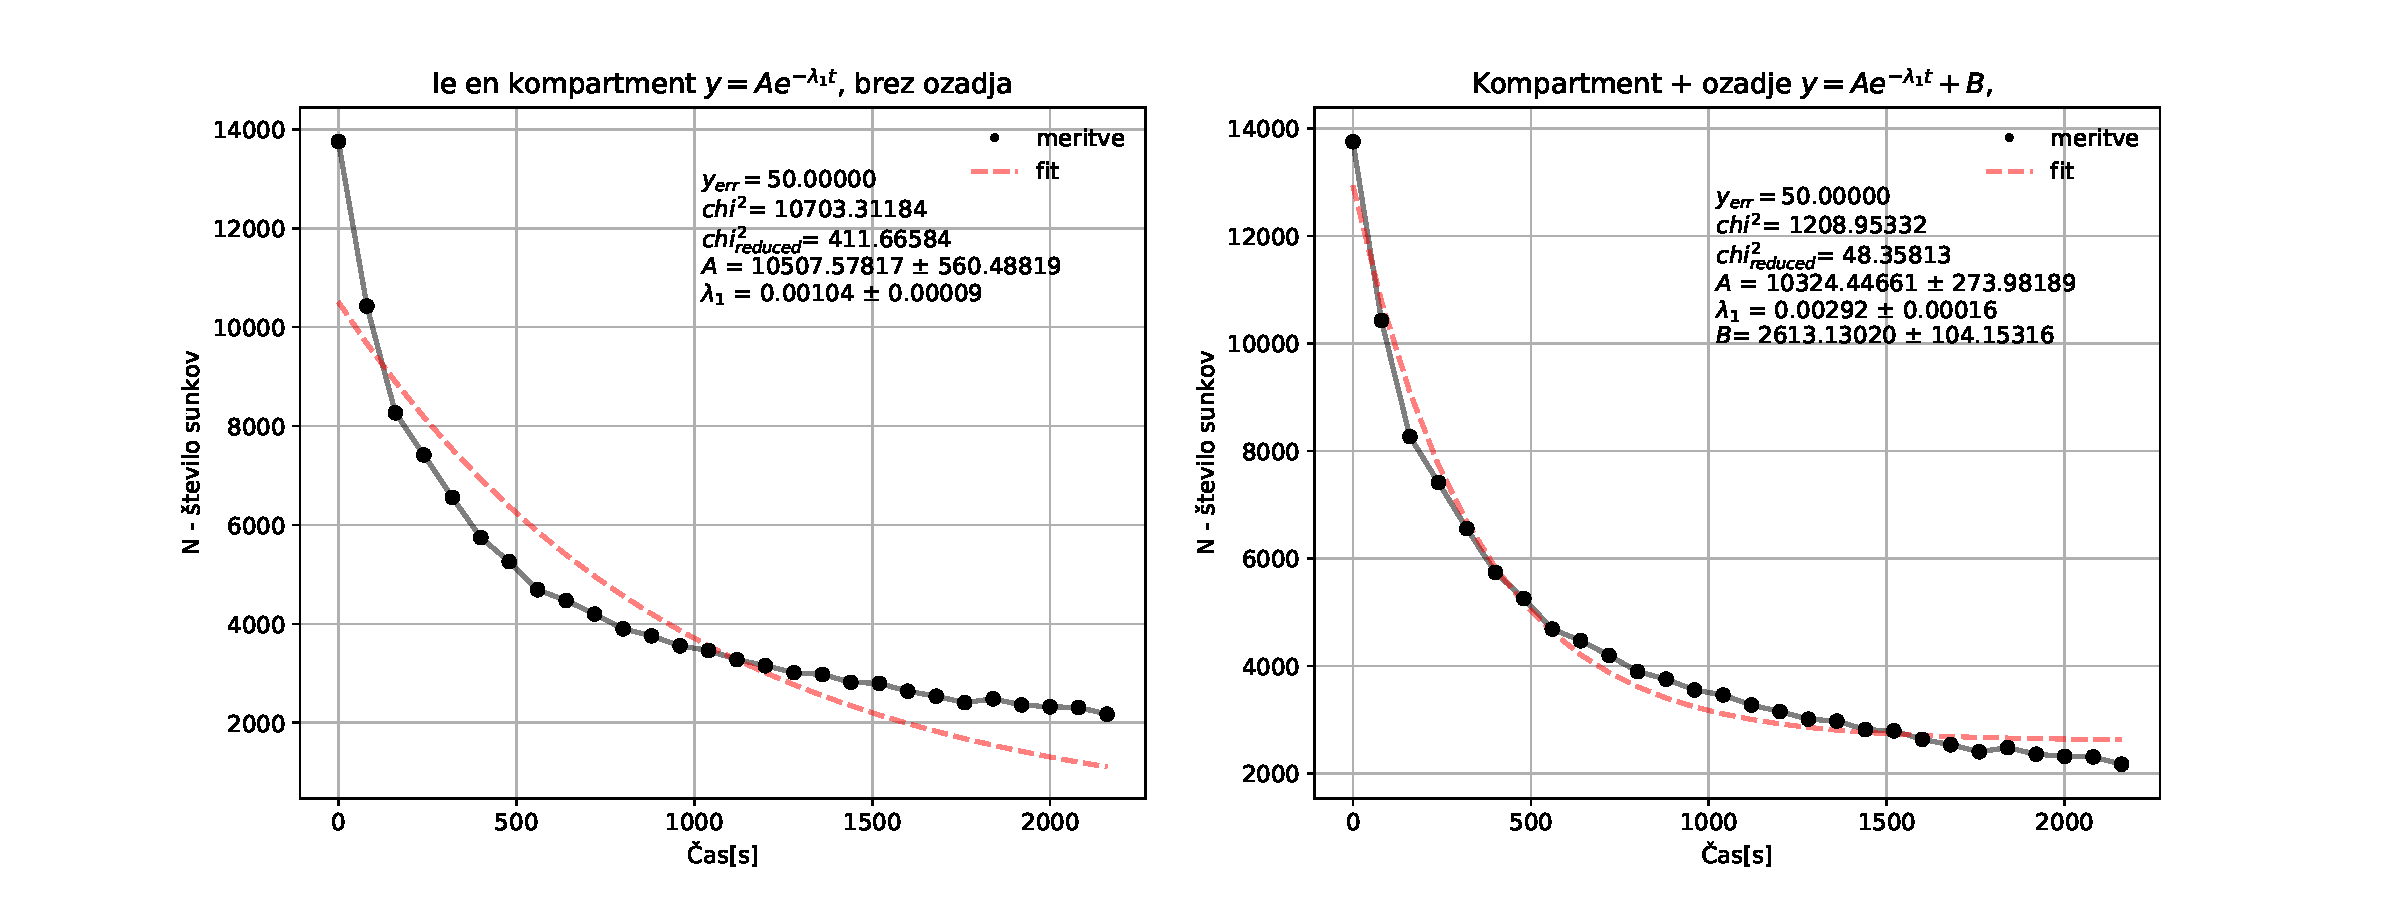
\includegraphics[width=24cm]{druga_en_kompartment.pdf}
 \caption{Osnovni model, ne more fitati eksponentne funkcije na naše podatke, zato dodamo ozadje na desni in vidimo veliko boljše prilagajanje in manjši $\chi^2$. Še vedno pa vidimo, da pri daljših časih, podatki ne sledijo začetnem modelu in zato naš razdelek sklopimo še z enim razdelkom. Desno dodamo v model konstani člen $B$ , ki opisuje sevanje iz ozadja.}
\end{figure}
Vidimo, torej da znaša ozadje približno 2500 fotonov. \newline
Poglejmo si napake fita, ki kažejo na to, da je model slab.
 \begin{figure}[H]
   
  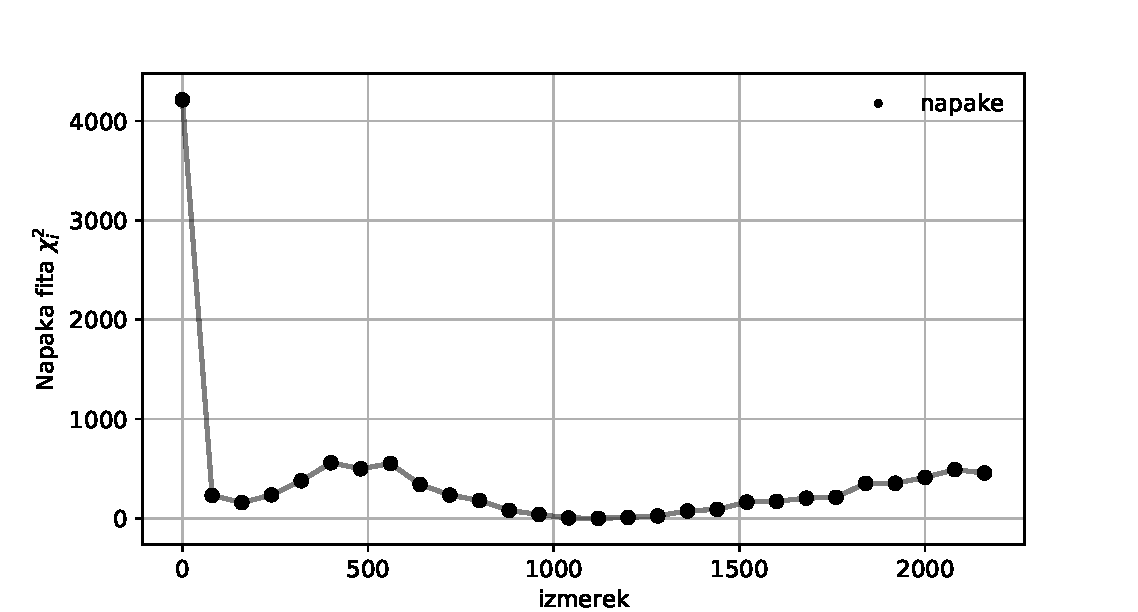
\includegraphics[width=16cm]{druga_napaka_1.pdf}
 \caption{Napaka osnovnega eno razdelčnega modela}
\end{figure}
 \begin{figure}[H]
   
  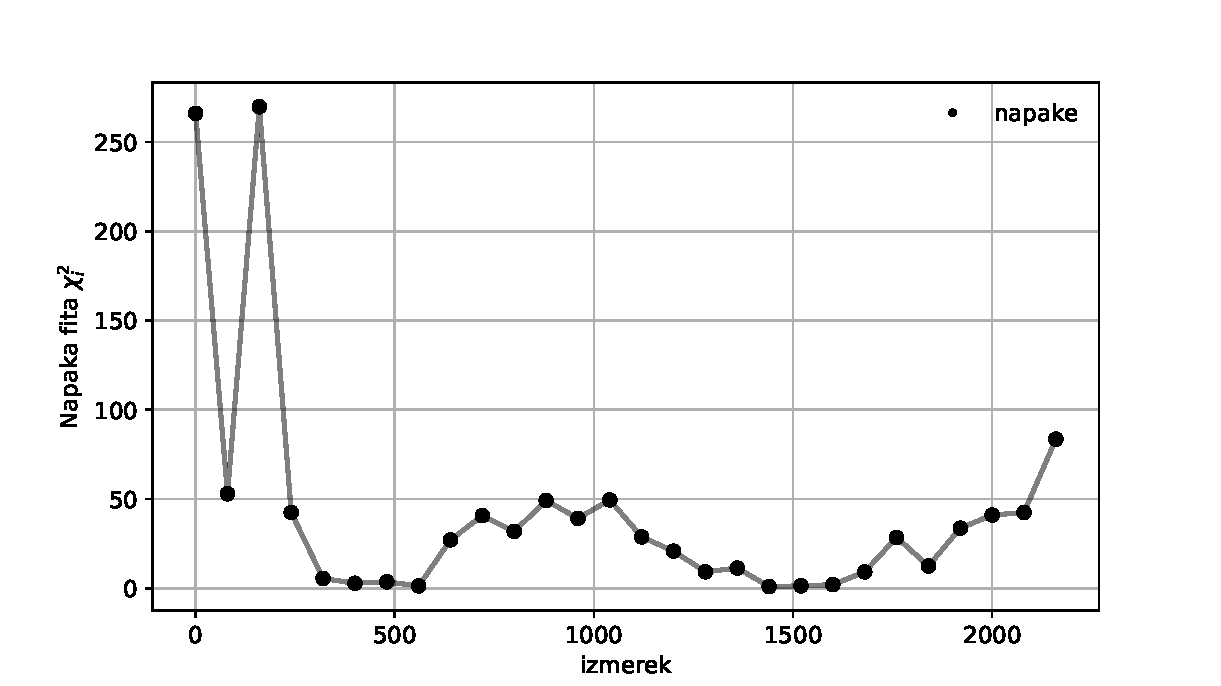
\includegraphics[width=16cm]{druga_napaka_2.pdf}
 \caption{Dodatek aditivne konstantne zelo zniža napake.}
\end{figure}
\subsection{Dvorazdelčen model}
Ker vemo, da je sistem ledvic kompleksen, dodajmo še kakšen razdelek, kamor lahko odteka hipuran.
\begin{equation}
\begin{split}
\dot{C_1} &= -\lambda C_1 -K_1 (C_1 - C_2) \\
\dot{C_2} &= +K_2 (C_1 - C_2), \\
\end{split}
\end{equation}
Vzemimo $K_1 = K_2$ in rešimo sistem, s nastavkom dveh eksponetnih funkcij.
\begin{equation}
\begin{split}
C_1 &= A e^{-\lambda_1 t} + B e^{-\lambda_2 t} \\ 
C_2 &= C e^{-\lambda_3 t} + D e^{-\lambda_4 t} \\ 
\end{split}
\end{equation}
Ali pa naredimo model, ki nekako upošteva difuzijo in tako opiše izgubo tekočine, kot $\sqrt{t}$
\begin{equation}
\begin{split}
C_1 &= A e^{-\lambda_1 \sqrt{t}} +B
\end{split}
\end{equation}
 \begin{figure}[H]
\hspace*{-2.5cm}     
  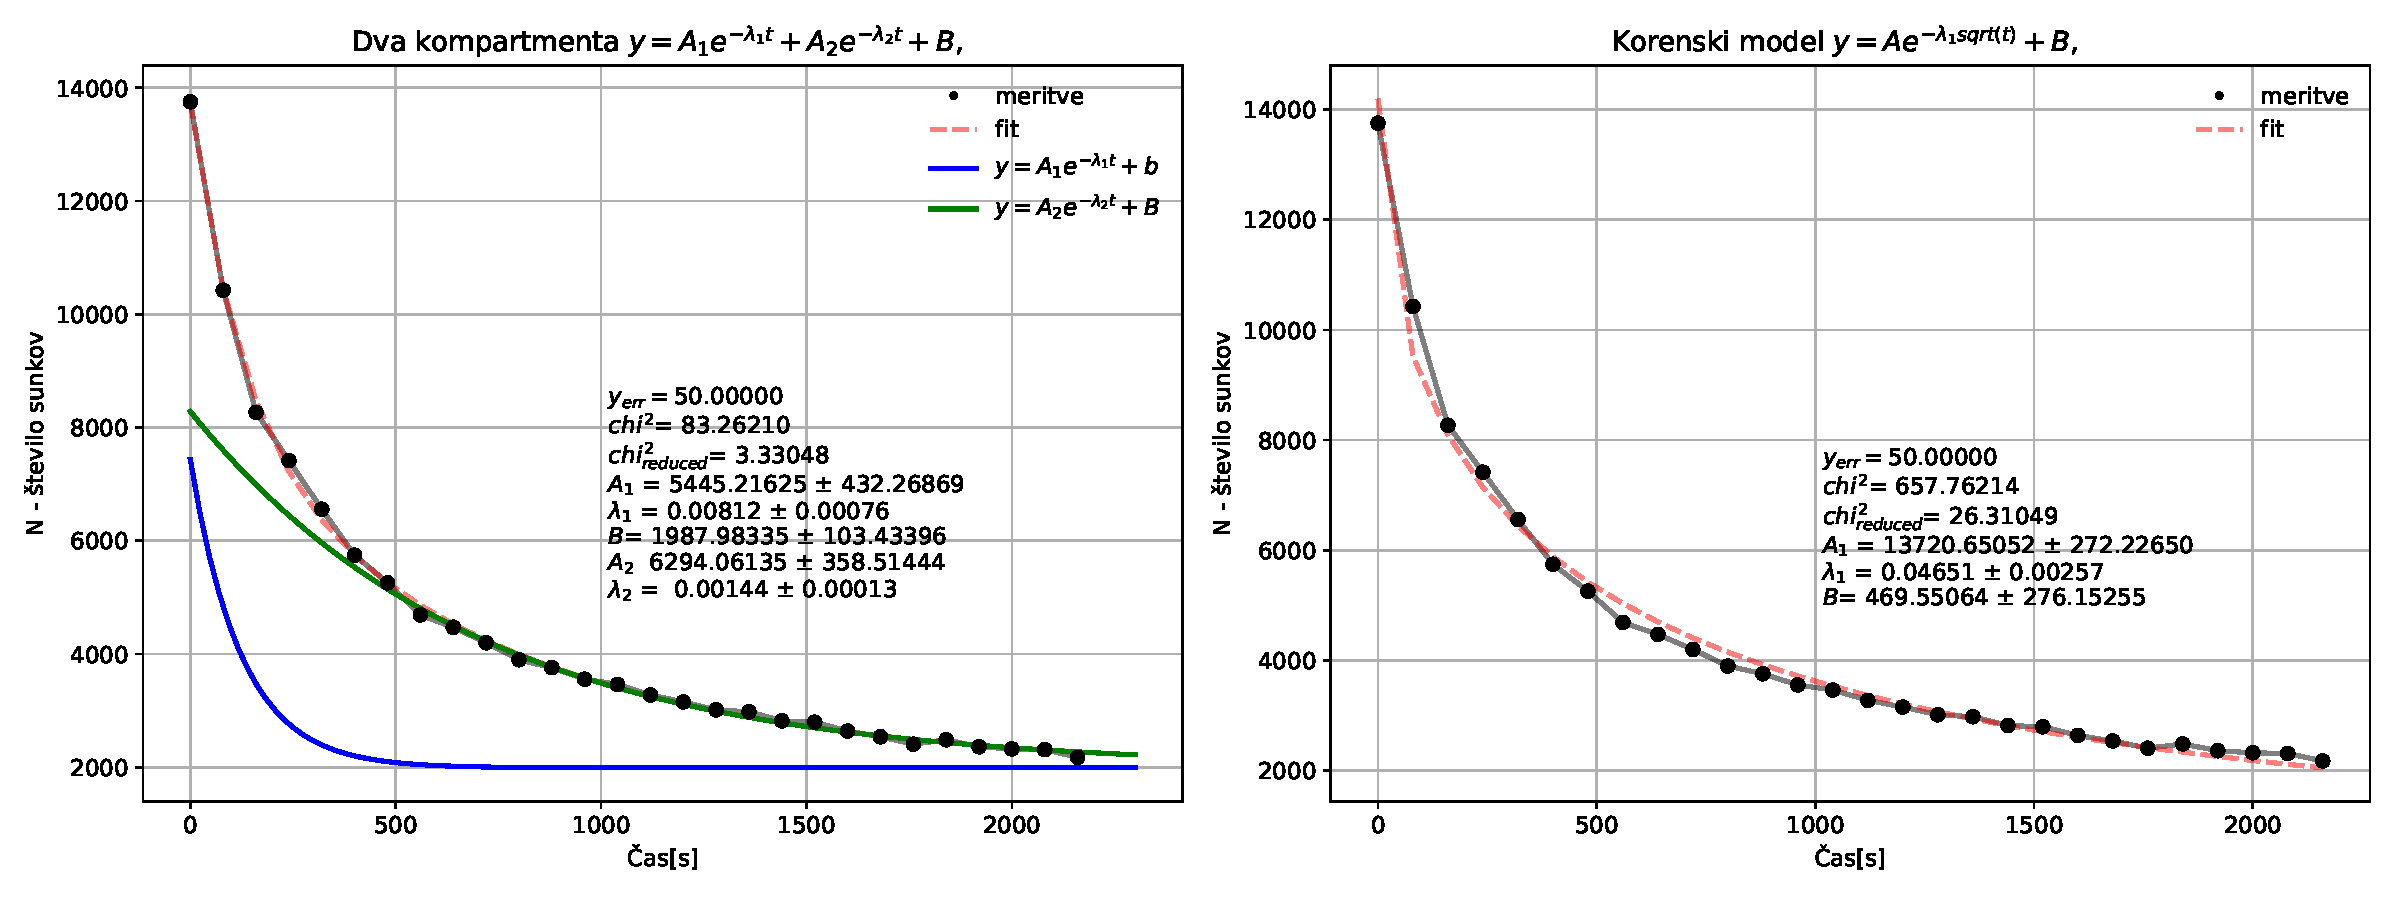
\includegraphics[width=20.cm] {druga_dva_kompartmenta.pdf}
 \caption{Fit s dvema kompartmentoma na levi nam $\chi^2$ zelo zmanjša in vidimo, da je fit dober. Na grafu vidimo tudi dva prispevka filtriranja hipurana, v prvi in drugi sistem, koncentracija drugega dela upade veliko hitreje, kot prvega in tako razdeli naš pretok na dva režima. Na desni pa je korenski fit, ki proti osnovnem eno-razdelčnem problemu precej izboljša fit. Začetni parametri so optimalni parametri iz slike (3), in vidimo, da parametri precej razlikuejjo od prejšnega modela, prav tako ozadje.  Poiskusil sem tudi dvo razdelčni korenski model $C_1 = A e^{-\lambda_1 \sqrt{t}} +B+  D e^{-\lambda_2 \sqrt{t}}$ , ki pa nam divergira za začetne približek uporabljen iz optimalnih parametrov osnovnega dvo-razdelčnega problema.}
\end{figure}
 \begin{figure}[H]
   
  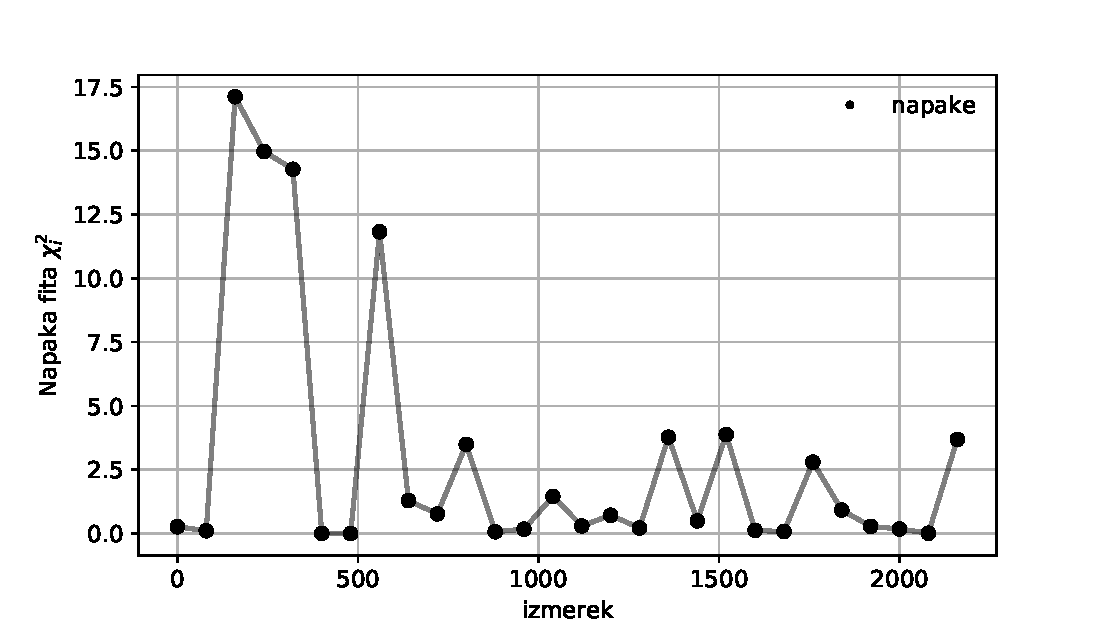
\includegraphics[width=16cm]{druga_napake_4.pdf}
 \caption{Napake dvo-razdelčnega modela so skoraj enakomerne in majhne.}
\end{figure}
Zapišimo tabelo, kjer so zapisani vsi $\chi^2$  in ugotovimo, da je najboljši model model dveh razdelkov.
\begin{table}[H]
  \begin{center}
    \caption{Vrednosti $\chi^2$ v odvisnosti od modela}
    \label{tab:table1}
    \begin{tabular}{l|c|r} % <-- Alignments: 1st column left, 2nd middle and 3rd right, with vertical lines in between
      \textbf{model} & \textbf{$\chi^2$}  & \textbf{$\chi_{reduced}^2$} \\
      \hline
      $C = A e^{-\lambda t}$ & 10 703 & 110\\
      $C = A e^{-\lambda t} + B$ & 1208 & 12 \\
     $C_1 = A e^{-\lambda_1 t} + B e^{-\lambda_2 t}$ & 83 &  0.882\\
     $C_1 = A e^{-\lambda_1 \sqrt{t}} +B$  & 657 & 6.7 \\
    \end{tabular}
  \end{center}
\end{table}
Iz podatkov $A,B,\lambda_1,\lambda_2$ lahko izračunamo čistilnost ledvic.
\section{Model korozije}
Ko površina kovine pride v stik z elektrolitom, zaradi razlik v kemijskih lastnostih posameznih področij kovine nastanejo mikrogalvanski členi, ki začnejo korozijo - anodnih in katodnih reakcij, kjer poteka oksidacije (oddajanje elektronov) in redukcije (sprejemanje elektronov). Tako se kovina po površini poškoduje in pridobi značilno rjasto barvo.
\subsection{Model korozije}
Parametre korozije določajo iz U-I diagrama med kovino in korozivnim elektrolitom, kjer zapišemo model
\begin{equation}
I = I_0 ( e^{\frac{U}{U_0}} - e^{-\frac{U}{U_c}})
\end{equation}


\begin{figure}[H]
\hspace*{-2.5cm}     
  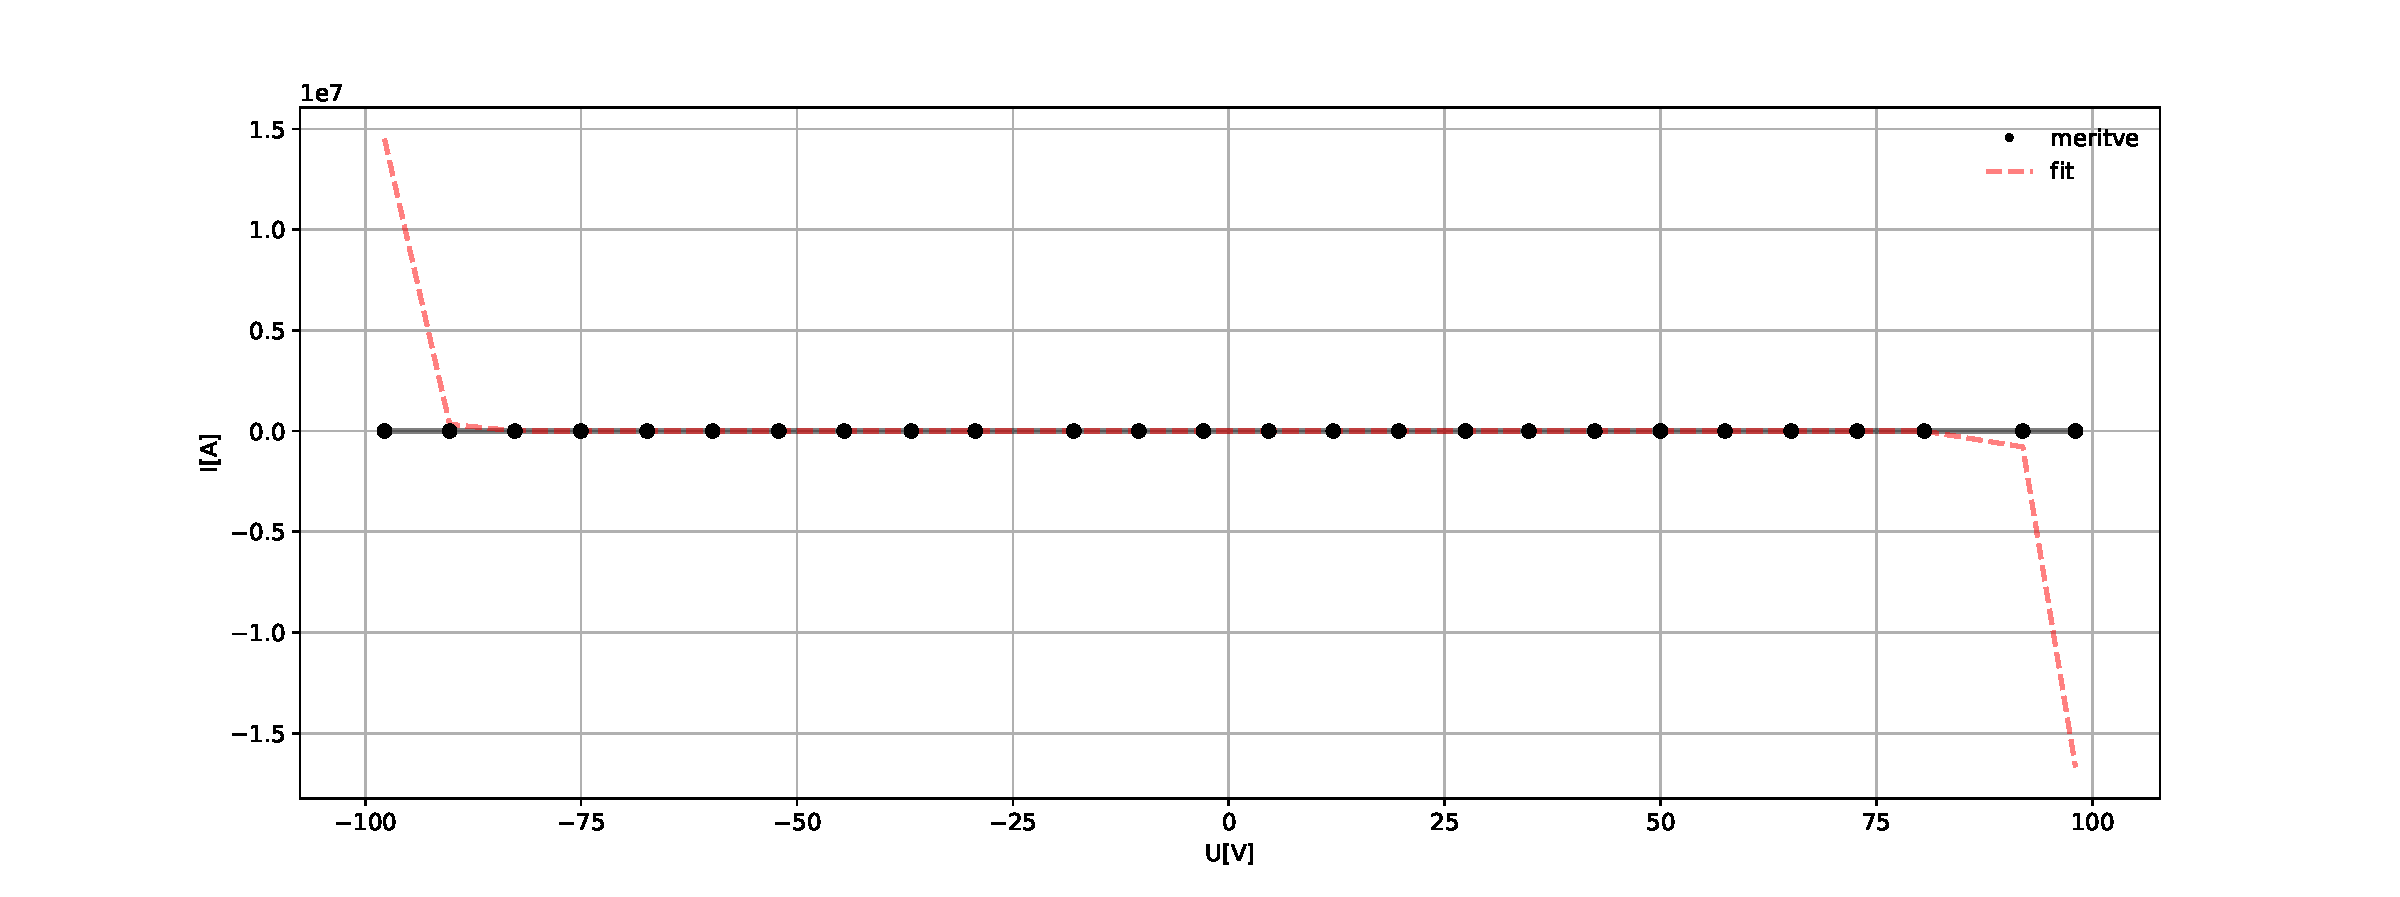
\includegraphics[width=20.cm] {tretja_slab_fit.pdf}
 \caption{Če ustavimo preprost začetni približek [1,1,1] se parametri ujamemjo v drug lokalni minimum.}
\end{figure}
Zaradi tega bom poiskusil na dva načina poiskati začetne parametre, ki nam bodo pomagali poiskati začetni približek.
\subsection{Normalizacija podatkov}
Najprej bom naše napetosti normaliziral okoli povprečja, tako da bodo meli varianco $\sigma$ enako 1.
\begin{equation}
x = \frac{x - \bar{x}}{\sigma}
\end{equation}
Uvedemo lahko tudi "reskaliranje", ki nam podatke transformira med [0,1].
\begin{equation}
 x={\frac {x-{\text{min}}(x)}{{\text{max}}(x)-{\text{min}}(x)}}
\end{equation}
tretja normalizacija pa je kombinacija obeh dveh.
\begin{equation}
 x_n={\frac {x-{\text{mean}}(x)}{{\text{max}}(x)-{\text{min}}(x)}}
\end{equation}
\begin{figure}[H]
\hspace*{-2.5cm}     
  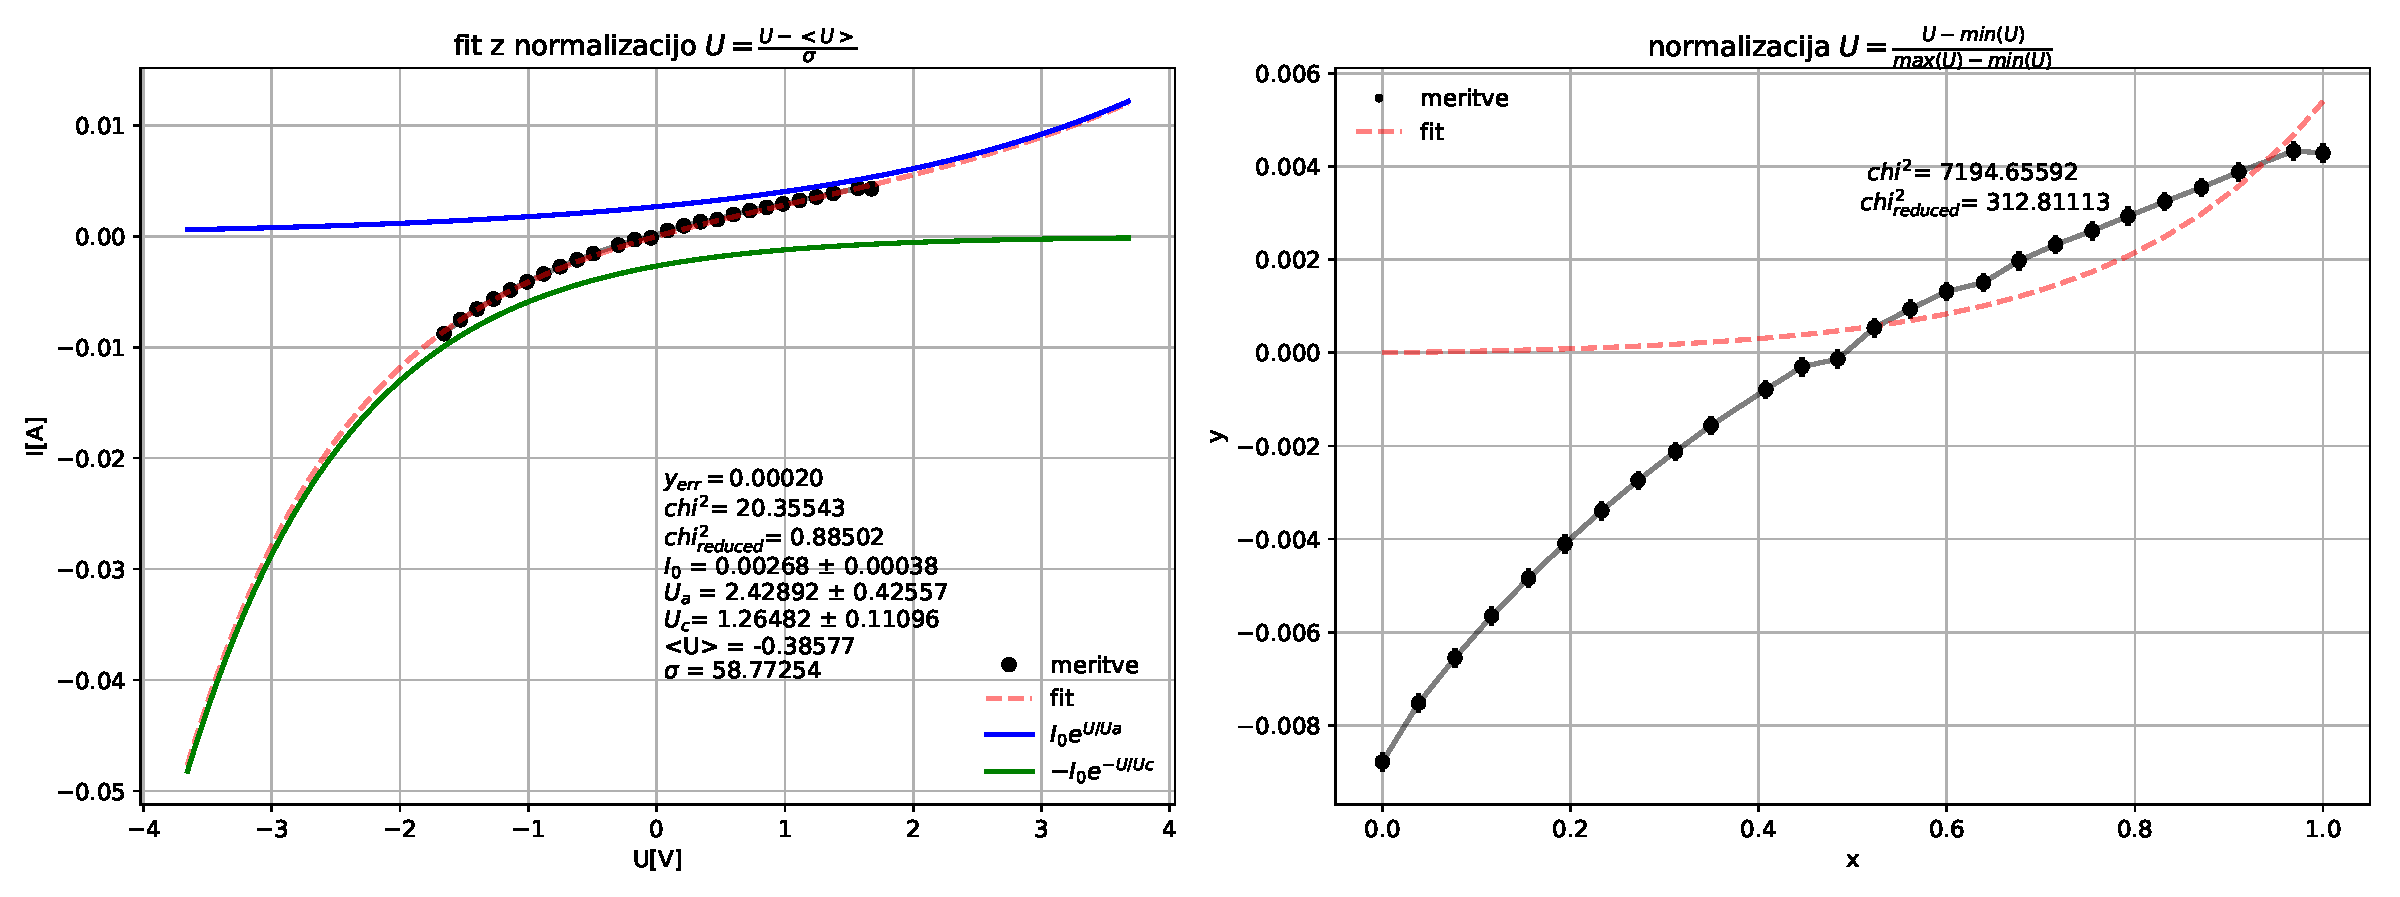
\includegraphics[width=20.cm] {tretja_normalizacija.pdf}
 \caption{Ko smo uvedli normalizacijo okoli povprečja (levo) nam je metoda za več različnih začetnih približkov skonvergirala v dober fit, pri reskaliranju (desno)pa ni pomagalo. }
\end{figure}
\begin{figure}[H]
\hspace*{-2.5cm}     
  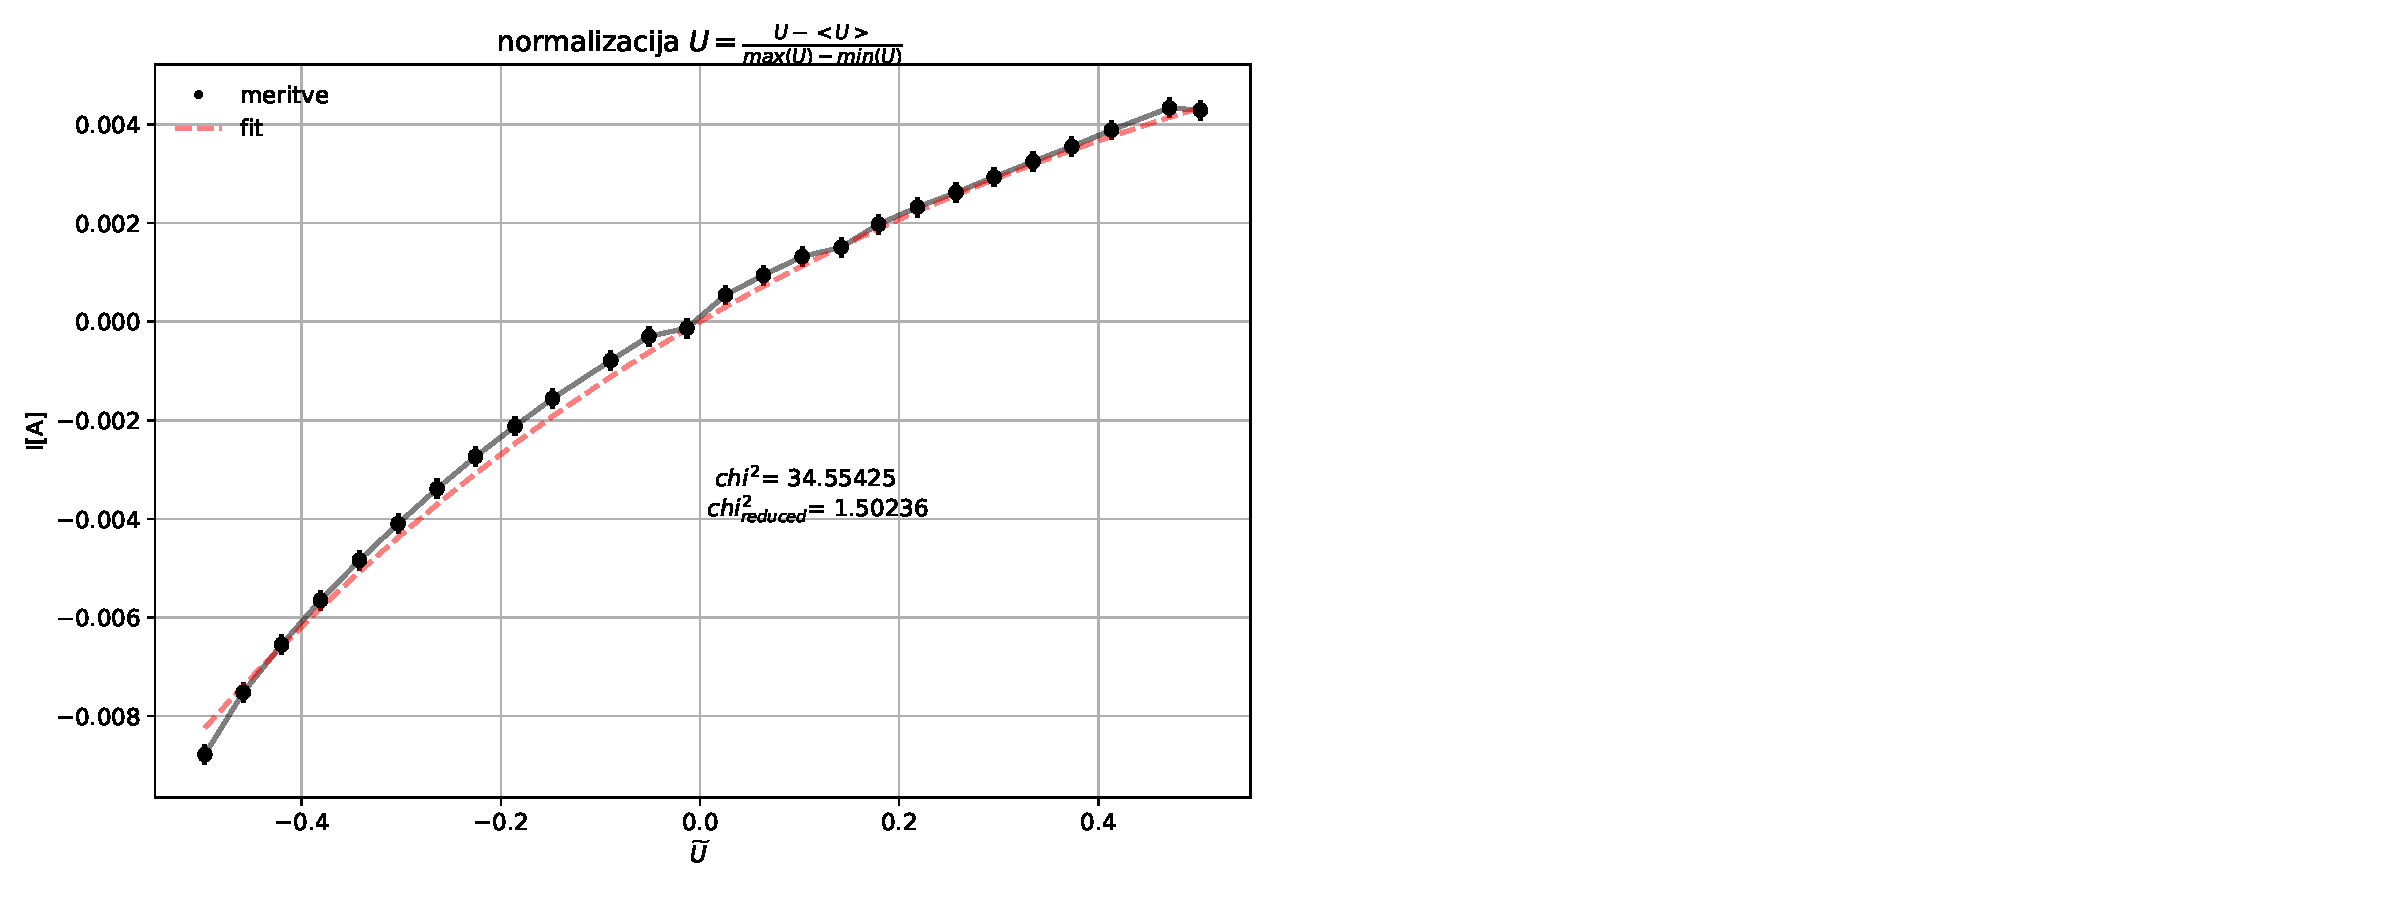
\includegraphics[width=20.cm] {tretja_normalizacijski_fit2.pdf}
 \caption{Pri normalizaciji med [-0.5,0.5] je  fit slabši, kot pri normalizaciji okoli povprečja.}
 \end{figure}
 Seveda optimalni parametri iz zgornjih rešitev niso isti kot v osnovnem modelu, saj smo jih prilagjali drugim podatkom. Če bi želeli le napovedovati, bi bili s tem zadovoljni, saj je važno da model prav napoveduje, vendar pa želimo dobiti točne parametre, da povemo nekaj o moči korozije, zato poskusimo te optimalne parametre uporabiti kot začetne približke na osnovnih podatkih, saj vemo, da so parametri v pravih razmerjih.
 \begin{figure}[H]
\hspace*{-3.5 cm}     
  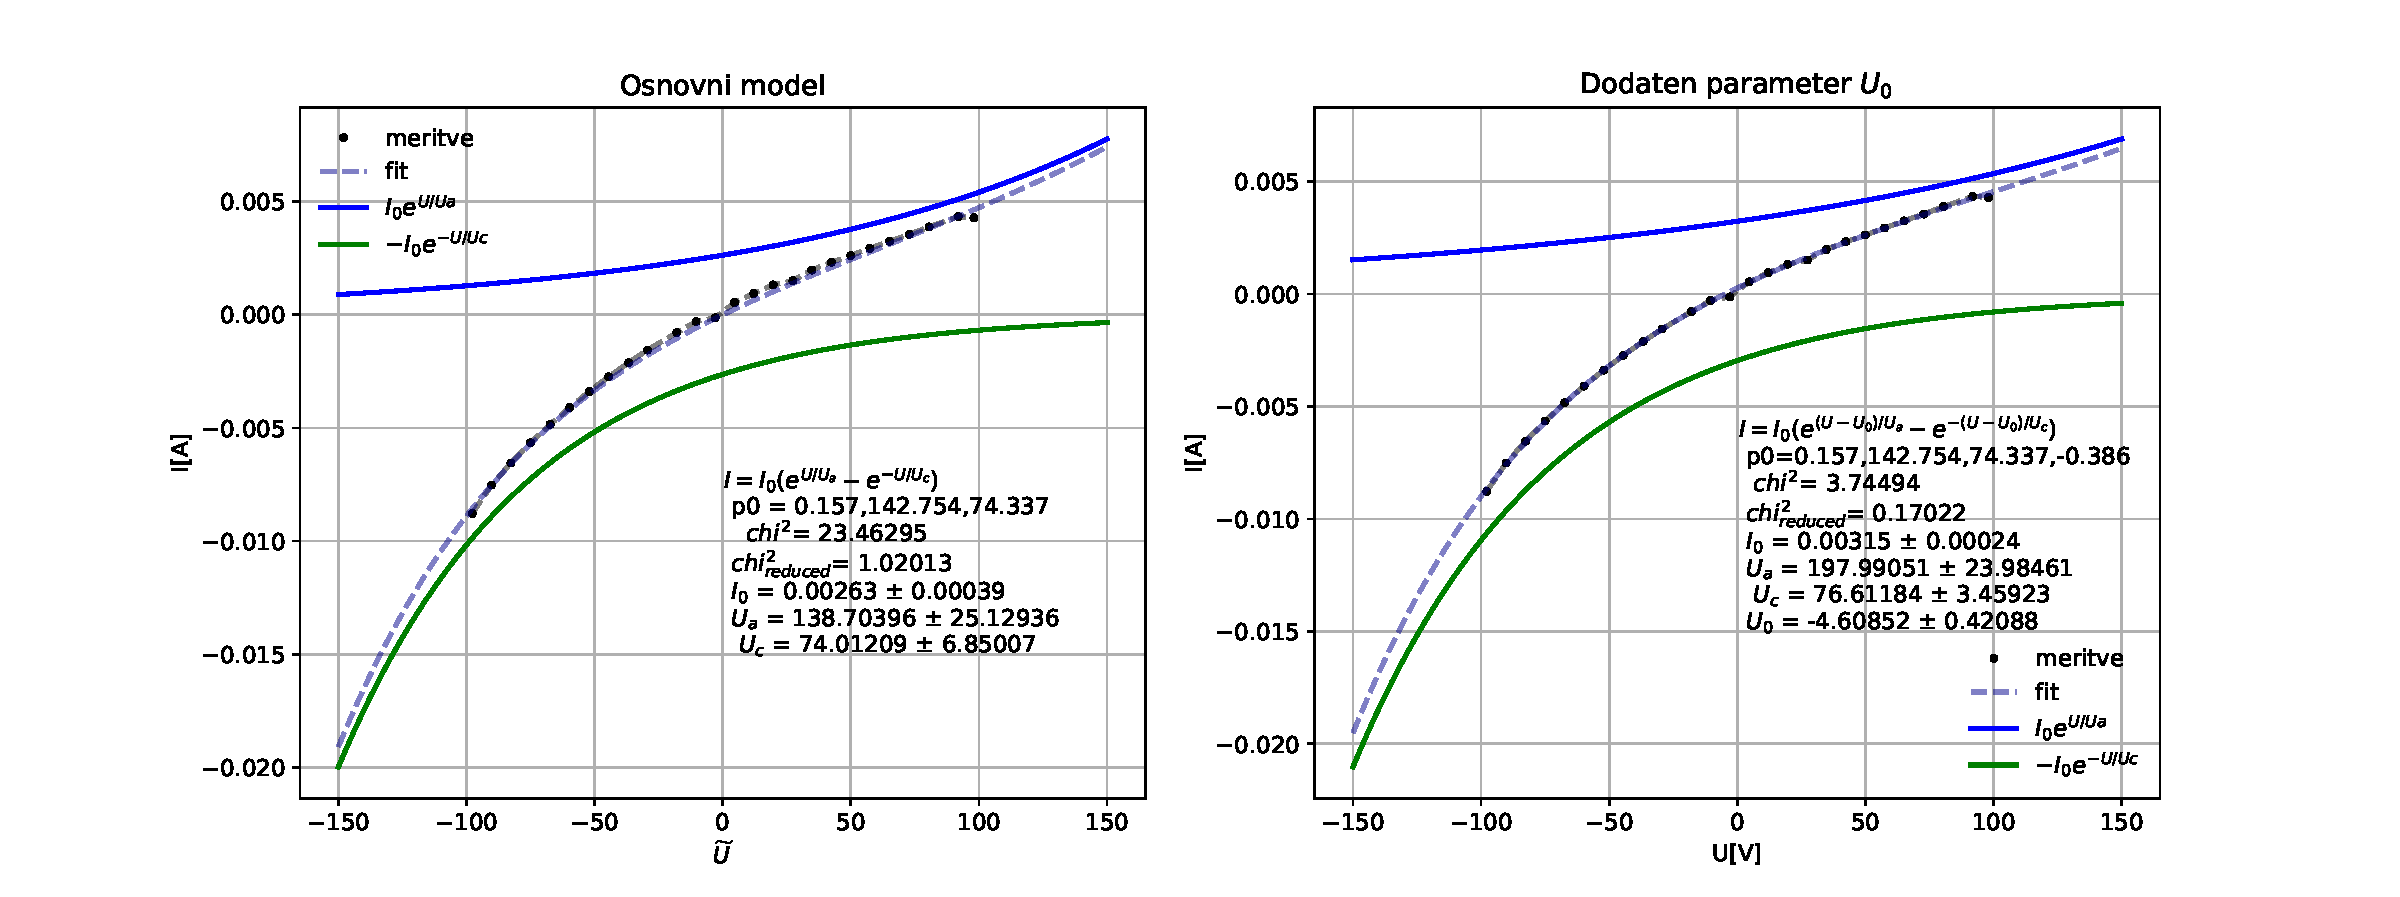
\includegraphics[width=24cm] {tretja_pravi_fit.pdf}
 \caption{Vidimo da smo z osnovnimi parametri iz normaliziranega modela zaradi enakega $I_0$ lahko našli minimum in tako dobro fitali model. Napaka, ki sem jo predpostavil je $y_{err} = 0.0002$. (desno) ker vemo, da voltmeter nikoli ni skalibriran okoli 0, uvedemo dodatni parameter $U_0$, ki nam premakne naš model, ter tako občutno zmanjšamo $\chi^2$. Tu vidimo, da so naše napake premajhne, saj je desni model zagotovo boljši. Napetosti so premaknjene za -4.6V. Na grafu je tudi narisan vsak eksponetni člen posebaj.}
 \end{figure}
 \textbf{ Kar vidimo je na desni zelo nizka vrednost $\chi^2_{reduced}$ , kar pomeni dvoje, ali da smo "over - fitali" , in se prilagodili točno na naše podatke, ali pa da je napaka premajhna in je zato tudi $\chi^2_{reduced}$  premajhen. Napako sem ocenil na  $0.0002 A$ kar je približno $10\%$. Druga možnost pa je da so napake podatkov še manjše in bi nam tako zvišale $\chi^2$. Ker je model fizikalno smiselen sumimo na drugo možnost in znižamo napake na $0.0001$, zaradi česar se $\chi^2_{reduced}$ zviša na $0.68$, kar pa je že bližje optimalnem.\newline\newline
 Narišimo še graf razlik fita z dodatnim parametrom $U_0$ in osnovnim modelom}
  \begin{figure}[H]
\hspace*{-3.5 cm}     
  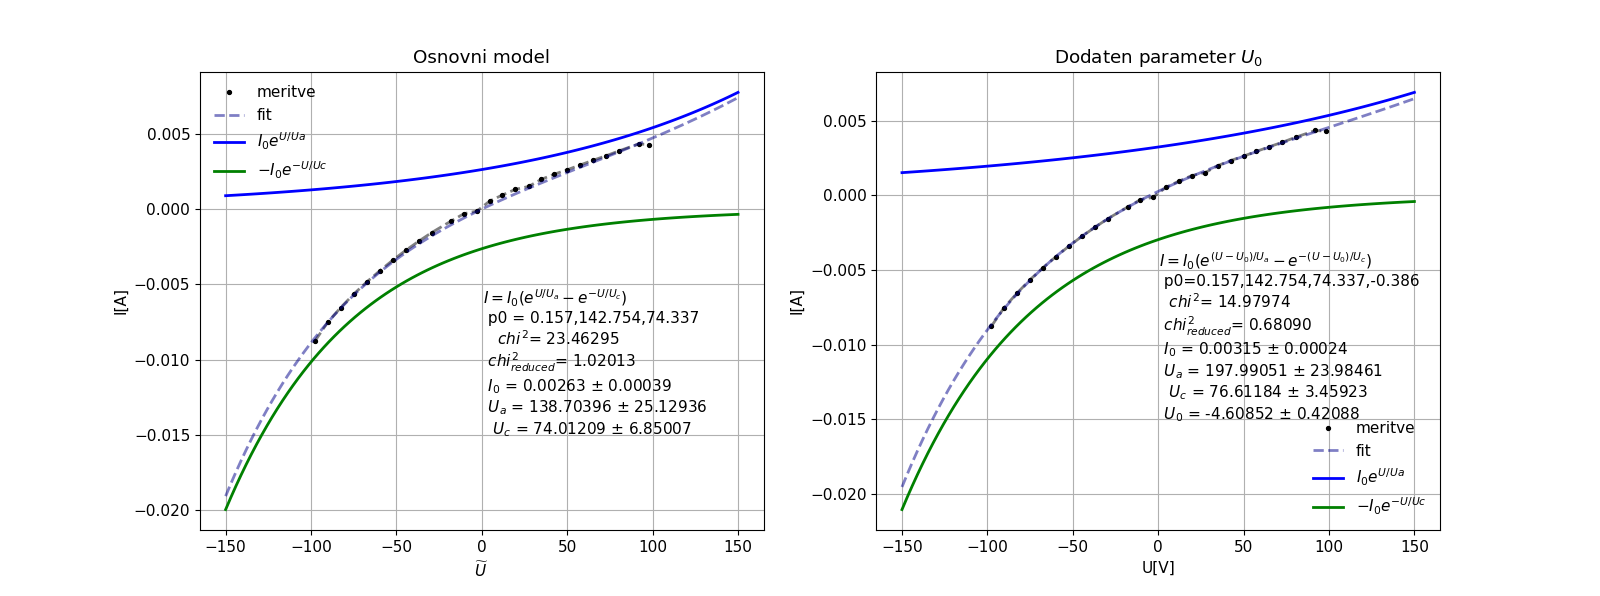
\includegraphics[width=24cm] {tretja_pravi_fit_zvisanje_chi.png}
 \caption{Napake yerr so se znižale na $0.0001$, ter tako uravnovesile $\chi^2$}
 \end{figure}
 
  \begin{figure}[H]
    
  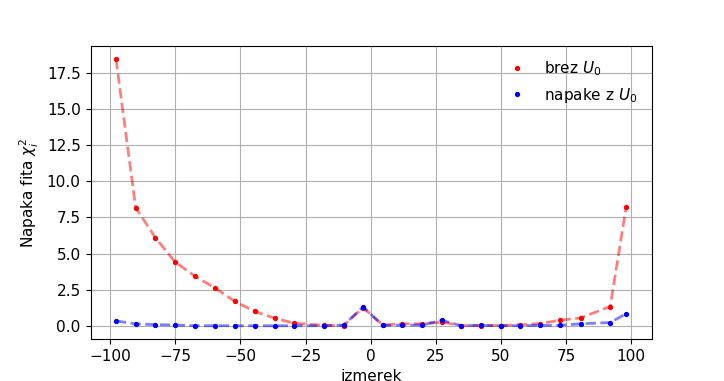
\includegraphics[width=15cm] {tretja_napaka_3.png}
 \caption{Razlike med fitom in podatki}
 \end{figure}

Sedaj lahko tudi razložimo model. S višanjem napetosti tok (modra), povezan z andodo in redukcijskimi reakcijami narašča, negativni tok, povezan s katodo pa pada. Tako pri $U>0$ en pri pri $U<0$ drug režim. Verjetno je tok močnejši/šibkejši gledena korozivnost materiala, kar pomeni da kovina odstopa od danega modela, ki smo ga naučili.
Če uporabimo za začetni približek optimalne parametre iz drugih normalizacij nam ti ne dajo rešitve. 
 \begin{figure}[H]
\hspace*{-3.5cm}     
  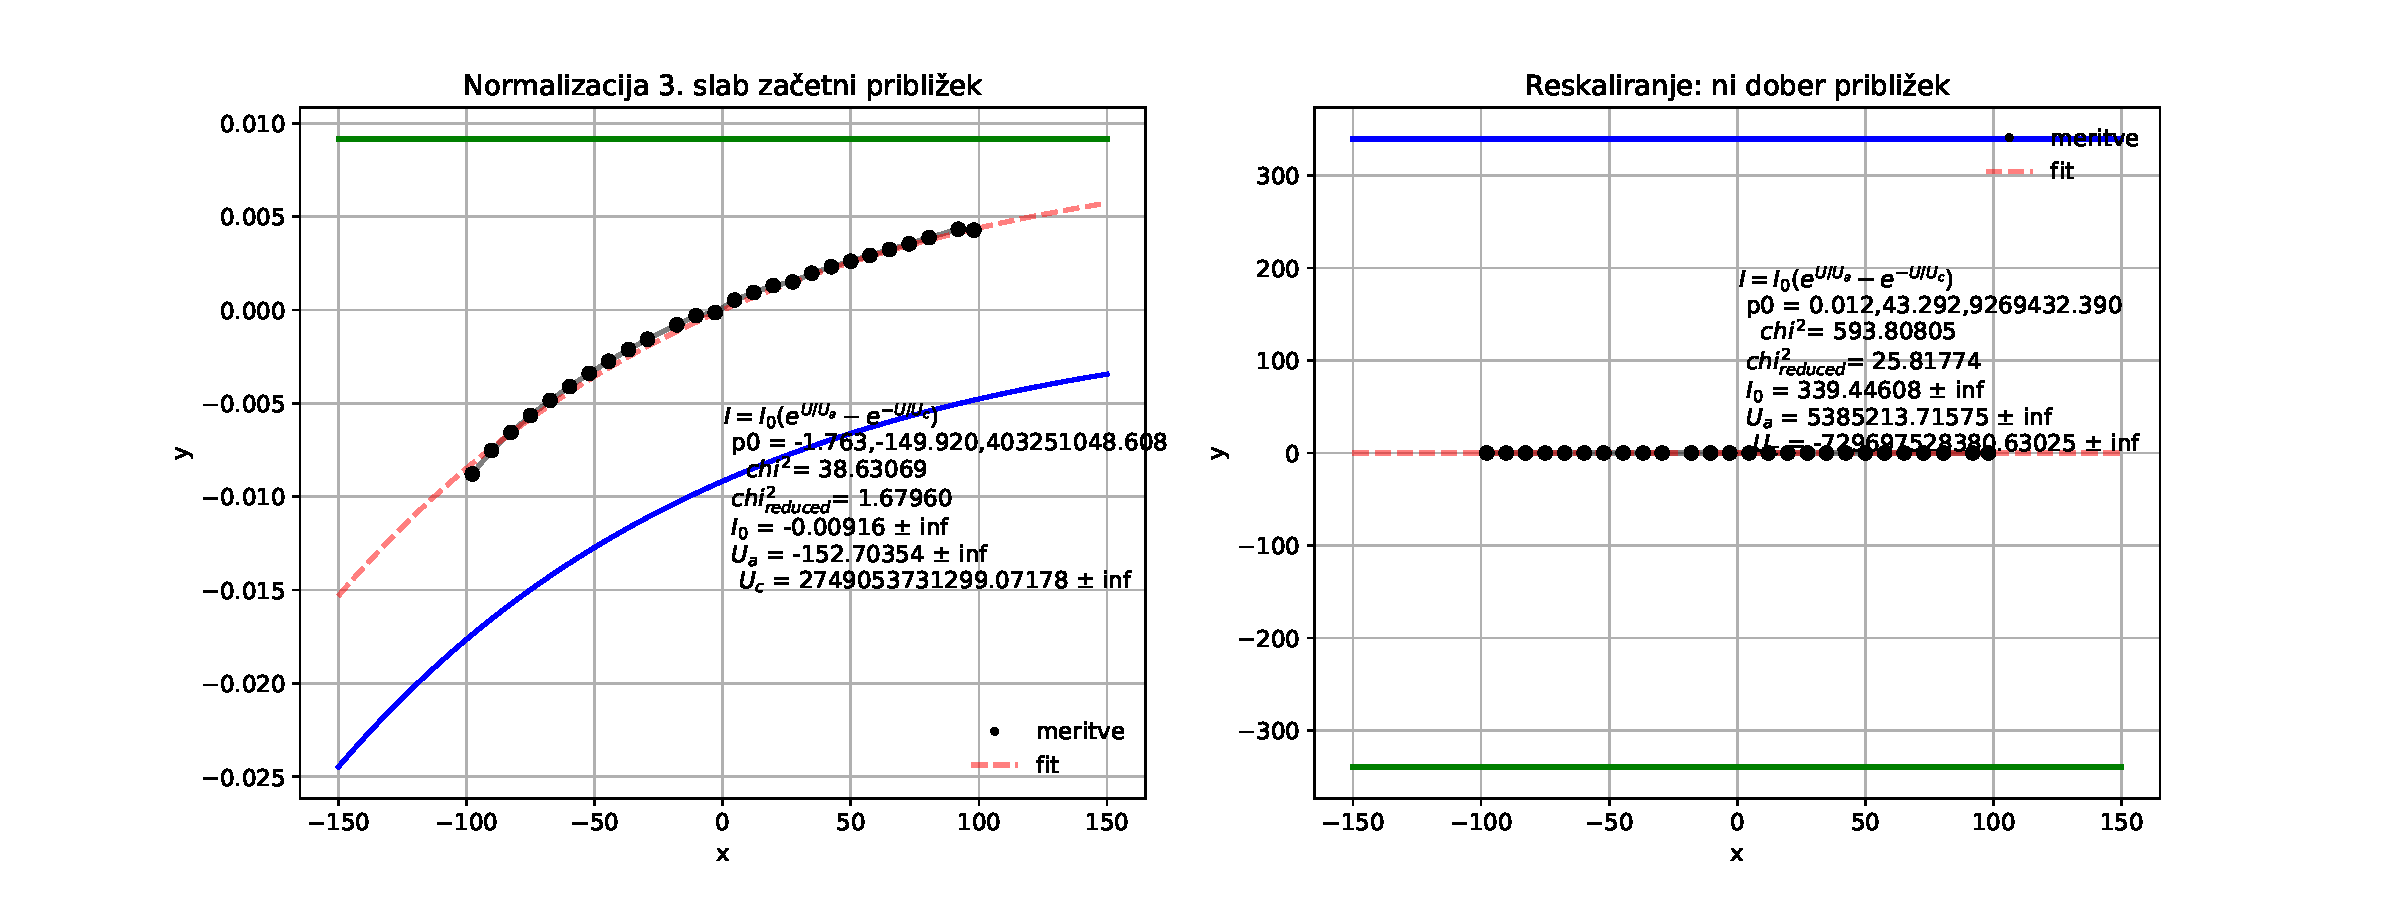
\includegraphics[width=24cm] {tretja_slab_fit2.pdf}
 \caption{Približek iz drugih oblik normalizacij ne deluje dobro.}
 \end{figure}
\subsection{Približna rešitev modela}
Fizikalno bomo dobre začetni približek našli tako, da najprej najdemo približni model, ki je manj občutljiv, kot eksponetni, zato model razvijemo
\begin{equation}
I = A U + B U^2 + C U^3
\end{equation}
kjer so $A,B,C$ neznane konstane.
Iz njih lahko izrazimo $I0,U_a,U_c$ in jih nato ustavimo kot začetni približek v osnovni model, ter tako dobimo

 \begin{figure}[H]
\hspace*{-3.5cm}     
  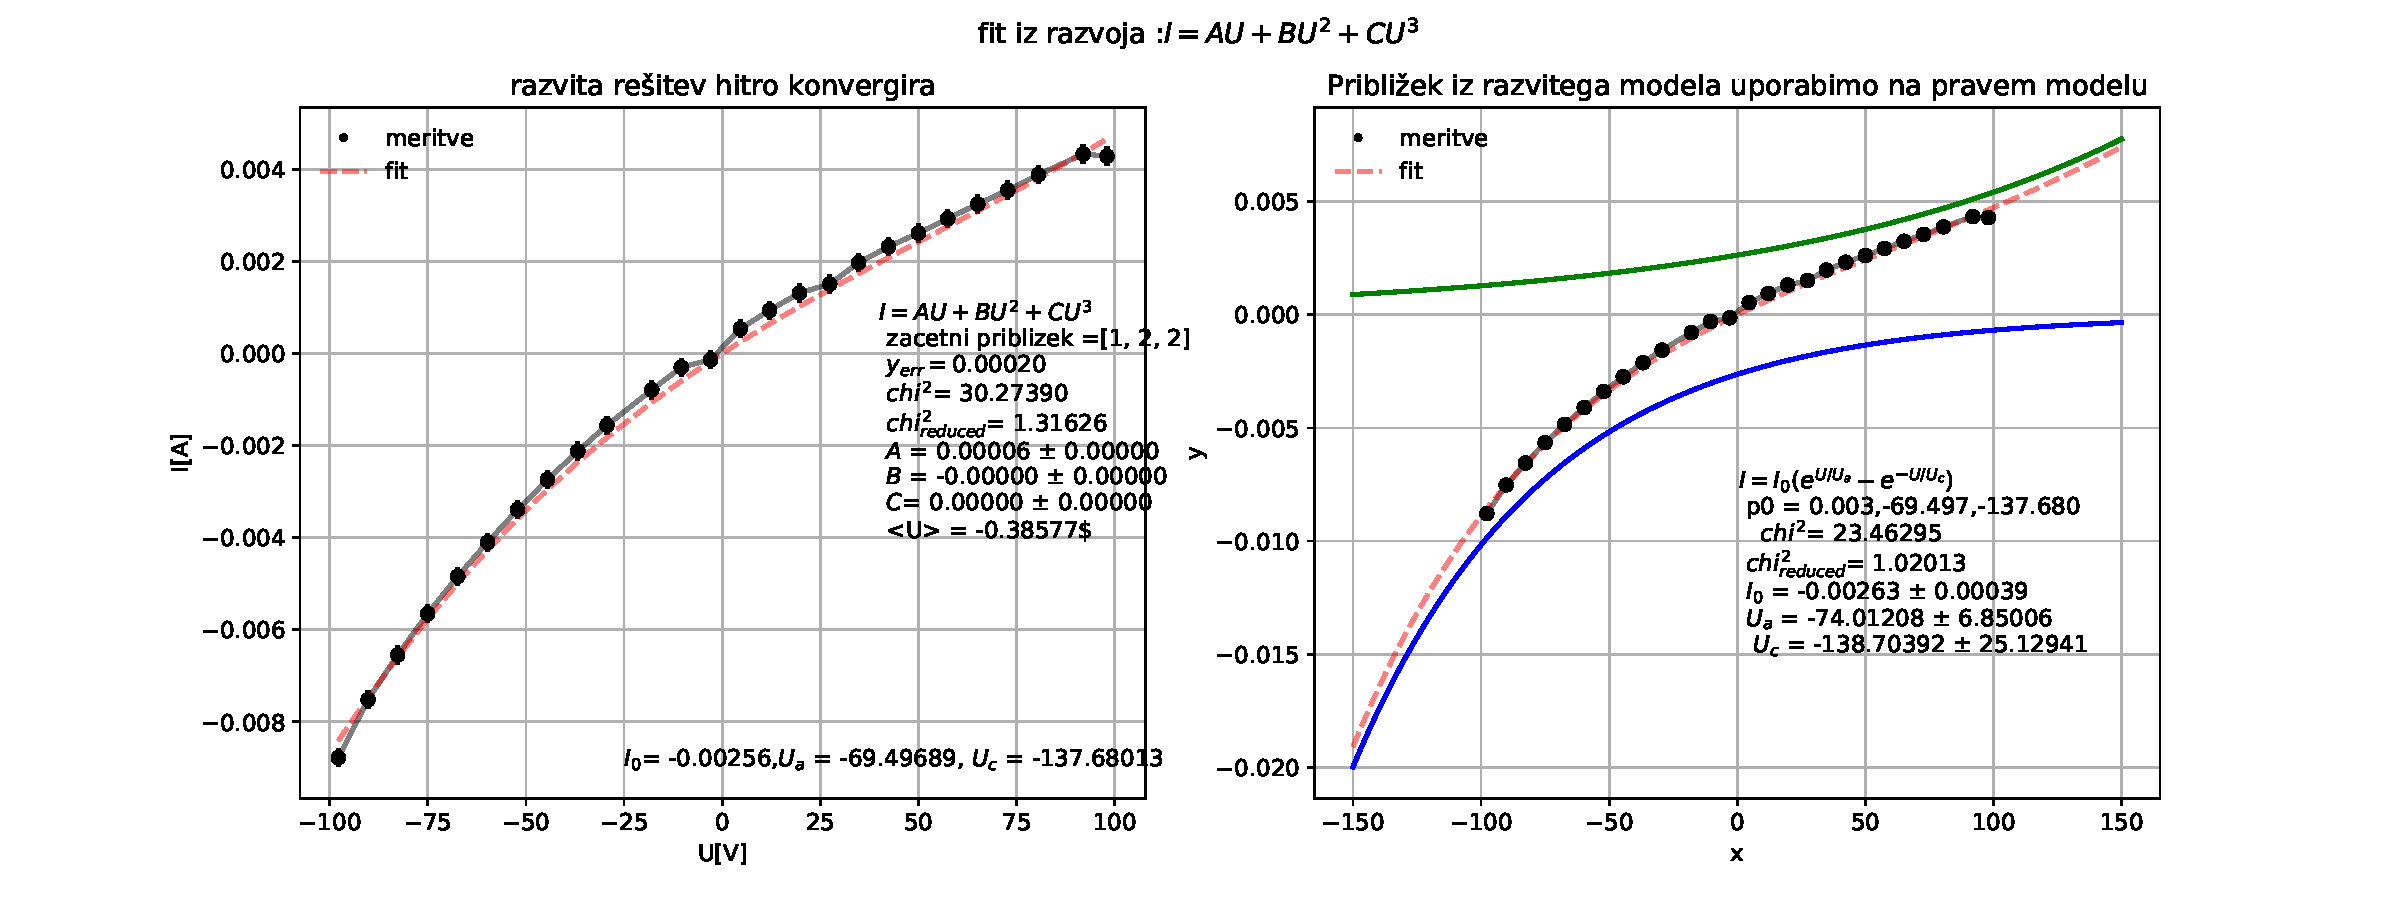
\includegraphics[width=24cm] {tretja_razvoj_fit.pdf}
 
 \end{figure}
Tako smo iz približne rešitve dobili dobro oceno za začetni približe.
\section{Zaključek}
Pogledali smo si kaj kako numerično poiskati optimalne parametre in kako zgradimo nelinearni model, ter koncept razdelčnih modelov, ki so zelo uporabni v medicini. S pomočjo modelov, lahko na na podlagi odstopanja novih meritev od modela, napovemo npr. ali so ledvica zdrava ali ne.
\end{document}